\documentclass{article}

\usepackage{pgfplots}

\usepgfplotslibrary{fillbetween}

\begin{document}

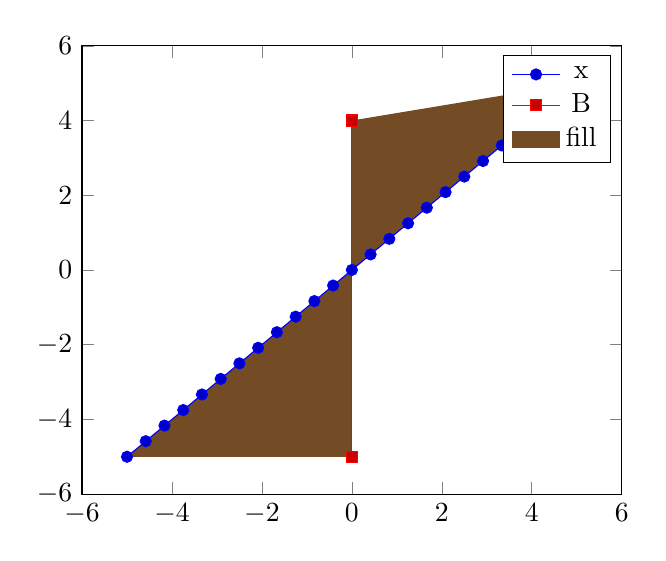
\begin{tikzpicture}
	\begin{axis}
	\addplot+[name path=A] {x};
	\addlegendentry{x}

	\addplot+[name path=B] coordinates {(0,-5) (0,4)};
	\addlegendentry{B}

	\addplot fill between[of=A and B];
	\addlegendentry{fill}
	\label{x}
	\end{axis}
\end{tikzpicture}

Das ist \ref{x}
\end{document}

